%---------------------------------------------------------------------------%
%-                                                                         -%
%-                          Beamer Template                                -%
%-                                                                         -%
%---------------------------------------------------------------------------%
%- Copyright (C) Huangrui Mo <huangrui.mo@gmail.com> 
%- This is free software: you can redistribute it and/or modify it
%- under the terms of the GNU General Public License as published by
%- the Free Software Foundation, either version 3 of the License, or
%- (at your option) any later version.
%---------------------------------------------------------------------------%
%->> Document class declaration
%---------------------------------------------------------------------------%
\documentclass[compress,table,aspectratio=169,xcolor={usenames,dvipsnames}]{beamer}%
%- Multiple options:
%- [<t|c|b>]% vertical alignment for content, vertically centered is default
%- [<slidestop|slidescentered>]% set frame titles position
%- [compress]% reduce the navigate bars
%- [<red|blue|brown|blackandwhite>]% set navigate bar color
%- [<10pt|11pt|12pt|14pt|17pt>]% set font size for normal text, 11pt is default
%- [table]% support tables
%- [aspectratio=169]% set aspect ratio to 16:9, and frame size to 160mm by 90mm
%- [aspectratio=1610]% set aspect ratio to 16:10, and frame size to 160mm by 100mm
%- [aspectratio=MN]% set aspect ratio to M:N, and frame size to 10*M mm by 10*N mm
%- [xcolor={usenames,dvipsnames}]% issue options to xcolor via a beamer-option
%- Manually adjust aspect ratio: design to 4x3, then expand to target, and live with empty space
%- \documentclass[aspectratio=169]{beamer}
%-     \beamertemplatenavigationsymbolsempty%
%-     \usepackage{pdfpages}%
%- \begin{document}
%-     \setbeamercolor{background canvas}{bg=}%
%-     \includepdf[pages=-]{my-original-presentation.pdf}%
%- \end{document}
%- The default font size may seem small, but the actual size of each frame size is
%- by default just 128mm by 96mm and the viewer application enlarges the frame and font.
%- By specifying a default font size smaller than 11pt one can put more onto each slide,
%- by specifying a larger font size one can fit on less.
%---------------------------------------------------------------------------%
%->> Document settings
%---------------------------------------------------------------------------%
\usepackage[biber,authoryear,tikz,table,xlink, fontspec, svg]{Style/artrabeamer}% document settings
\setsansfont{Europa-Regular}
%- usage: \usepackage[option1,option2,...,optionN]{artrabeamer}
%- Multiple optional arguments:
%- [CJK]% Chinese environment support
%- [bibtex|biber]% set bibliography processor and package
%- [<numbered|authoryear|alpha>]% set citation and reference style
%- <numbered>: textual: Jones [1]; parenthetical: [1]
%- <authoryear>: textual: Jones (1995); parenthetical: (Jones, 1995)
%- <alpha>: textual: not available; parenthetical: [Jon95]
%- [tikz]% provide complex diagrams via tikz package
%- [table]% provide complex tables via ctable package
%- [list]% provide enhanced list environments for algorithm and coding
%- [math]% enable some extra math packages
%- [showonlynote]% show note pages only
%- [showsecnote]% show note pages on second screen
%- [handout]% enable handout output
%- [xlink]% disable link colors
\usepackage{Style/artracom}% user defined commands
%---------------------------------------------------------------------------%
%->> Document inclusion
%---------------------------------------------------------------------------%
%\includeonly{Tex/Sec_Introduction}% selected files compilation
%\includeonlylecture{lecture label}% selected lectures compilation
%---------------------------------------------------------------------------%
%->> Theme settings
%---------------------------------------------------------------------------%
%-
%-> Recommended theme combinations
%-
%- set: [<usetheme>, <useoutertheme>, <useinnertheme>, <usecolortheme>]
%- light: [<CambridgeUS>, <miniframes>, <circle>, <dove|seahorse|beaver|seagull>]
%- light: [<Boadilla|Madrid>, <default>, <circle>, <dove|seahorse|beaver|seagull>]
%- dark: [<Boadilla|Madrid>, <default>, <circle>, <fly|albatross>]
%-
%-> Global themes
%-
\usetheme{CambridgeUS}%
%- Options:
%- [<Boadilla|CambridgeUS|default|...>]
%- It is the complete theme in the sense that they control just about every aspect
%- of a slide's appearance. Think of it as major theme.
%- Theme Matrix (https://www.hartwork.org/beamer-theme-matrix/) contains the
%- various theme and color combinations included with beamer.
%-
%-> Outer themes
%-
%\useoutertheme{}%
%- Options:
%- [<default|infolines|miniframes|smoothbars|sidebar|split|shadow|tree|smoothtree>]
%- An outer theme dictates (roughly) the overall layout of frames. It specifies where
%- any navigational elements should go (like a mini table of contents or navigational
%- mini frames) and what they should look like. Typically, an outer theme specifies
%- how the following elements are rendered:
%- - The headline and footline.
%- - The sidebars.
%- - The logo.
%- - The frame title.
%- The Beamer User Guide explains each theme with examples.
%-
%- *** Miniframes
\useoutertheme[%
    %footline=empty,% suppressed the footline (default).
    %footline=authorinstitute,% shows the author's name and the institute in the footline.
    %footline=authortitle,% shows the author's name and the title in the footline.
    %footline=institutetitle,% shows the institute and the title in the footline.
    %footline=authorinstitutetitle,% shows all three in the footline.
    subsection=false,% shows or suppresses line showing the subsection in the headline.
]{miniframes}%
%-
%- *** Sidebar
%\useoutertheme[%
%    %left,% sidebar links.
%    %right,% sidebar rechts.
%    %hideallsubsections,% suppresses all subsections.
%    %hideothersubsections,% suppresses all subsections except the current one.
%]{sidebar}%
%-
%-> Inner themes
%-
\useinnertheme{circles}%
%- Options:
%- [<default|circles|rectangles|rounded|inmargin>]
%- An inner theme installs templates that dictate how the following elements are typeset:
%- - Title and part pages.
%- - Itemize environments.
%- - Enumerate environments.
%- - Description environments.
%- - Block environments.
%- - Theorem and proof environments.
%- - Figures and tables.
%- - Footnotes.
%- - Bibliography entries.
%-
%-> Color themes
%-
\usecolortheme{dove}%
%- Options:
%- [<dove|seahorse|beaver|seagull|fly|albatross|...>]
%- Control the colors of title, frame title, itemization bullets,
%- and many other elements of a slide show.
%- More detailed configure:\setbeamercolor{beamer_element}{color} for
%- of Beamer elements, e.g.color setup
%\setbeamercolor{title}{fg=red!80!black,bg=red!20!white}
%\setbeamercolor{frametitle}{fg=blue,bg=yellow}
%---------------------------------------------------------------------------%
%->> Configuration
%---------------------------------------------------------------------------%
%-
%-> Set templates
%-
%- As a user of the beamer class you typically do not 'use' or 'invoke'
%- templates yourself, directly. For example, the frame title template
%- is automatically invoked by beamer somewhere deep inside the frame
%- typesetting process. The same is true of most other templates.
%- However, if, for whatever reason, you wish to invoke a template
%- yourself, you can use the following command.
%-\setbeamertemplate{some beamer element}{your definition for this template}
%-
%- *** Headline and footline
%\setbeamertemplate{headline}[infolines theme]
%\setbeamertemplate{footline}{\insertframenumber}
%- Options: {},[default],[infolines theme],[miniframes theme],[frame number],
%-          [page number],[text line]{ text },...
%- Example for redefine the footline:
%-
%- First define some "beamer color" entries:
%\setbeamercolor{myentry1}{fg=black,bg=red!20}
%\setbeamercolor{myentry2}{fg=black,bg=red!30}
%\setbeamercolor{myentry3}{fg=black,bg=red!40}
%- Syntax for \begin{beamercolorbox}[options]{beamer color} ... \end{beamercolorbox}.
%- footline:
\setbeamertemplate{footline}{
  \leavevmode%
  \hbox{%
  \begin{beamercolorbox}[wd=.5\paperwidth,ht=5ex,dp=2ex,left]%
    \\${}$\hspace*{2em}Digitec Galaxus AG%
  \end{beamercolorbox}%
  \begin{beamercolorbox}[wd=.5\paperwidth,ht=5ex,dp=2ex,right]%
    \\${}$Monatlicher Rückblick VPM | \insertframenumber{} / \inserttotalframenumber\hspace*{2em}
  \end{beamercolorbox}}%
  \vskip0pt%
}
%- headline:
%\setbeamertemplate{headline}{
%  \leavevmode%
%  \hbox{%
%  \begin{beamercolorbox}[wd=.5\paperwidth,ht=2.65ex,dp=1.5ex,right]{myentry1}%
%    \usebeamerfont{section in head/foot}\insertsectionhead\hspace*{2ex}
%  \end{beamercolorbox}%
%  \begin{beamercolorbox}[wd=.5\paperwidth,ht=2.65ex,dp=1.5ex,left]{myentry3}%
%    \usebeamerfont{subsection in head/foot}\hspace*{2ex}\insertsubsectionhead
%  \end{beamercolorbox}}%
%  \vskip0pt%
%}
%- Change the footer/footline of a single frame in Beamer: use {} to confine effect domain.
%- The \leavevmode ensures that the vertical mode is ended and horizontal mode is entered. 
%- In vertical mode, TeX stacks horizontal boxes vertically, whereas in horizontal mode, 
%- they are taken as part of the text line. Use \leavevmode for all macros which could be 
%- used at the begin of the paragraph and add horizontal boxes by themselves.
%-
%- *** Outline setting
%\AtBeginPart% [<Lecture|Part|Section>]% insert content at the beginning of each element
%{%
%    \frame[plain]{\partpage}% [<partpage|sectionpage>][<\insertlecture|\insertpart|\insertsection>]
%    \begin{frame}[plain]%
%        \frametitle{Outline}%
%        {%
%            \tableofcontents[sectionstyle=show/shaded,subsectionstyle=show/show/shaded]%
%        }%
%    \end{frame}%
%}
%- - sectionstyle=<style for current section>/<style for other sections>
%- - subsectionstyle=<style for current subsection>/<style for other
%-   subsections in current section>/<style for subsections in other sections>
%- - Allowed <styles> are show, shaded, and hide.
%- Other options:
%- - currentsection, equal to: sectionstyle=show/shaded,subsectionstyle=show/show/shaded
%- - currentsubsection, equal to: subsectionstyle=show/shaded.
%- - firstsection=<section number> specifies which section should be numbered as section "1."
%-   This is useful if you have a first section (like an overview section) that should not
%-   receive a number.
%- - hideallsubsections, equal to: subsectionstyle=hide.
%- - pausesections, causes a \pause command to be issued before each section.
%-   This is useful if you wish to show the table of contents in an incremental way.
%-
%- *** Navigation symbols
\setbeamertemplate{navigation symbols}{}% suppresses all navigation symbols.
%\setbeamertemplate{navigation symbols}[only frame symbol]% only for navigating frames.
%-
%- *** Frame title
%\setbeamertemplate{frametitle}[default][left]% left, center, right
%-
%- *** Background
%\setbeamertemplate{background}[grid][step=\grid,color=blue]
%\setbeamertemplate{background canvas}[default]
%\setbeamertemplate{background canvas}[vertical shading][bottom=red!20,top=yellow!30]
%\setbeamertemplate{background canvas}{\includegraphics[width=\paperwidth,height=\paperheight]{alps.jpg}}
%\tikzart[t=c]{cover_front_thu_cce}
%\tikzart[t=c]{cover_composite_tonemapped}[trim=0mm 100mm 0mm 0mm,clip]
%- The aspect ratio of a Beamer slide is 4:3 therefore it's best
%- if your background image has the same aspect ratio. Otherwise
%- your image will be distorted when it's stretched to cover the
%- slide from edge to edge.
%- To limit the background setting to a single slide, enclose the
% \setbeamertemplate{background canvas}{...} command in braces,
%- as in:
%-
%{% brace to limit the scope of \setbeamertemplate
%\setbeamertemplate{navigation symbols}{}% optionally hide navigation buttons
%\setbeamertemplate{background canvas}{\includegraphics
%	[width=\paperwidth,height=\paperheight]{alps.jpg}}
%\begin{frame}[plain]
%...
%\end{frame}
%}% closing brace
%-
%- *** Margin sizes
%\setbeamersize{text margin left=2em,text margin right=2em}
%-
%- *** Itemizations, enumerations, and descriptions
%\setbeamertemplate{itemize items}[triangle]
%- Options: [<circle|triangle|square|ball>].
%\setbeamertemplate{enumerate items}[default]
%- Options:
%- [default]% numbered
%- [sections numbered]% section numbered, subsections are not numbered.
%- [subsections numbered]% subsections are numbered, but not the sections.
%- [circle]% numbered circles before section, not subsection.
%- [square]% numbered squares before section. unnumbered squares before subsections.
%- [ball]% similar to square, but use balls.
%- [ball unnumbered]% similar to ball, except that no numbering is used.
%-
%- *** Block environments
%\setbeamertemplate{blocks}[rounded][shadow=true]
%- Types:
%- "theorem", "corollary", "definition" in structure color frame.
%- "examples" in green color frame.
%- "block" in structure color frame with your own title.
%- "alertblock" in alert color frame with your own title.
%-
%- *** Theorem environments
%\setbeamertemplate{theorems}[normal font]
%- Options: [<default|normal font|numbered|ams style>].
%-
%- *** Figures and tables
%\setbeamertemplate{caption}[default]
%- Options:
%- [default]% typesets the caption name (a word like 'Figure' or 'Abbildung' or 'Table')
%- [numbered]% adds the figure or table number to the caption.
%- [caption name own line].
%-
%- *** Adding sections and subsections
%\setbeamertemplate{sections/subsections in toc}[square]
%- Options: [<default|sections numbered|subsections numbered>]
%-          [<circle|square|ball|ball unnumbered>]
%-
%- *** Bibliography
%\setbeamertemplate{bibliography item}{}% remove the icon
%-
%-> Fonts
%-
%- Set fonts used for different elements of a slide via Beamer's Font Management.
%- Rules:
%\setbeamerfont{some beamer element}{size=\large}
%- Add * to the command to first completely "reset" the font attributes.
%- Options:
%- parent=structure,size=\large,series=\bfseries,shape=\itshape,family=\sffamily.
%- Explains: there are three familis of font
%- family: \rmfamily(serif) or \sffamily(sans serif), or \ttfamily(monospace).
%- Each family has its own font characteristics, i.e., font properties.
%- shapes: \itshape, \slshape, \scshape, or \upshape.
%- series(light, bold,...): \bfseries, \mdseries.
%-
%- *** Structure font
%\setbeamerfont{structure}{}
%\setbeamerfont{tiny structure}{size=\tiny}
%-
%- *** Normal font
%\setbeamerfont{normal text}{parent=structure,size=\small}% ignored currently
%\setbeamerfont{alerted text}{}
%\setbeamerfont{example text}{}
%-
%- *** Projected text font
%\setbeamerfont{projected text}{parent={tiny structure}}
%-
%- *** Titlepage font
%\setbeamerfont{title}{parent=structure, size=\large}% shape=\itshape,family=\rmfamily
%\setbeamerfont{title in head/foot}{parent=title, size=\tiny}
%\setbeamerfont{subtitle}{parent=title, size=\normalsize}
%\setbeamerfont{author}{parent=title, size=\normalsize}
%\setbeamerfont{author in head/foot}{parent=title, size=\tiny}
\setbeamerfont{institute}{parent=structure, size=\normalsize, series=\mdseries}
%\setbeamerfont{institute in head/foot}{parent=title, size=\tiny}
%\setbeamerfont{date}{parent=institute}
%\setbeamerfont{date in head/foot}{parent=title, size=\tiny}
%-
%- *** Frame title font
\setbeamerfont{frametitle}{parent=structure,size=\large}
%\setbeamerfont{framesubtitle}{parent=frametitle,size=\footnotesize}
%-
%- *** Part fonts
%\setbeamerfont{part name}{size=\Large}
%\setbeamerfont{part title}{parent=title}
%-
%- *** Headline and footline font
%\setbeamerfont{headline}{parent={tiny structure}}
%\setbeamerfont{footline}{parent={tiny structure}}
%-
%- *** Caption font
%\setbeamerfont{caption}{size=\small}
%\setbeamerfont{caption name}{size=\small}
%-
%- *** Button font
%\setbeamerfont{button}{size=\tiny}
%-
%-> Transparent effect
%-
%\setbeamercovered{invisible}
%- Options:
%- [invisible]% is the default and causes covered text to disappear.
%- [transparent]% creates shaded instead of hidden overlays.
%- [dynamic]% makes all covered text quite transparent, but in a dynamic way.
%- [highly dynamic]% has the same effect as dynamic, but the effect is stronger.
%\beamerdefaultoverlayspecification{<+->}% uncover everything in a step-wise fashion
%---------------------------------------------------------------------------%
%->> Document content
%---------------------------------------------------------------------------%
%-
%-> Titlepage information
%-
%---------------------------------------------------------------------------%
%->> Document inclusion
%---------------------------------------------------------------------------%
%\includeonly{Tex/Sec_Introduction,Tex/Sec_Method,Tex/Sec_Result,Tex/Sec_Conclusion}% selected files compilation
%\includeonlylecture{lec_present_intro,lec_present_method,lec_present_result,lec_present_conclude}% selected lectures compilation
%\includeonlyframes{fra_current}% selected frames compilation
%---------------------------------------------------------------------------%
%->> Titlepage information
%---------------------------------------------------------------------------%
\setbeamerfont{title}{size=\Huge}
\title[]% optional, abbreviated title
{\enorcn{Rückblick VPM}{}}

\date[]{\enorcn{01.05.2023 - 31.10.2023}{}}% or simply: \date{\today}
%\date[IDS 2018]{International Detonation Symposium, 2018}% conference name

%\subject{\enorcn{Report by Huangrui Mo}{}}% inserted into the PDF information catalog

%\logo{\tikzart[t=p,x=8,y=-6,w=4]{logo_uw}}% on each slide 
%\titlegraphic{\tikzart[t=p,x=0,y=0]{logovpm}}% only on title page

\titlegraphic{
  \hspace*{-7mm}
  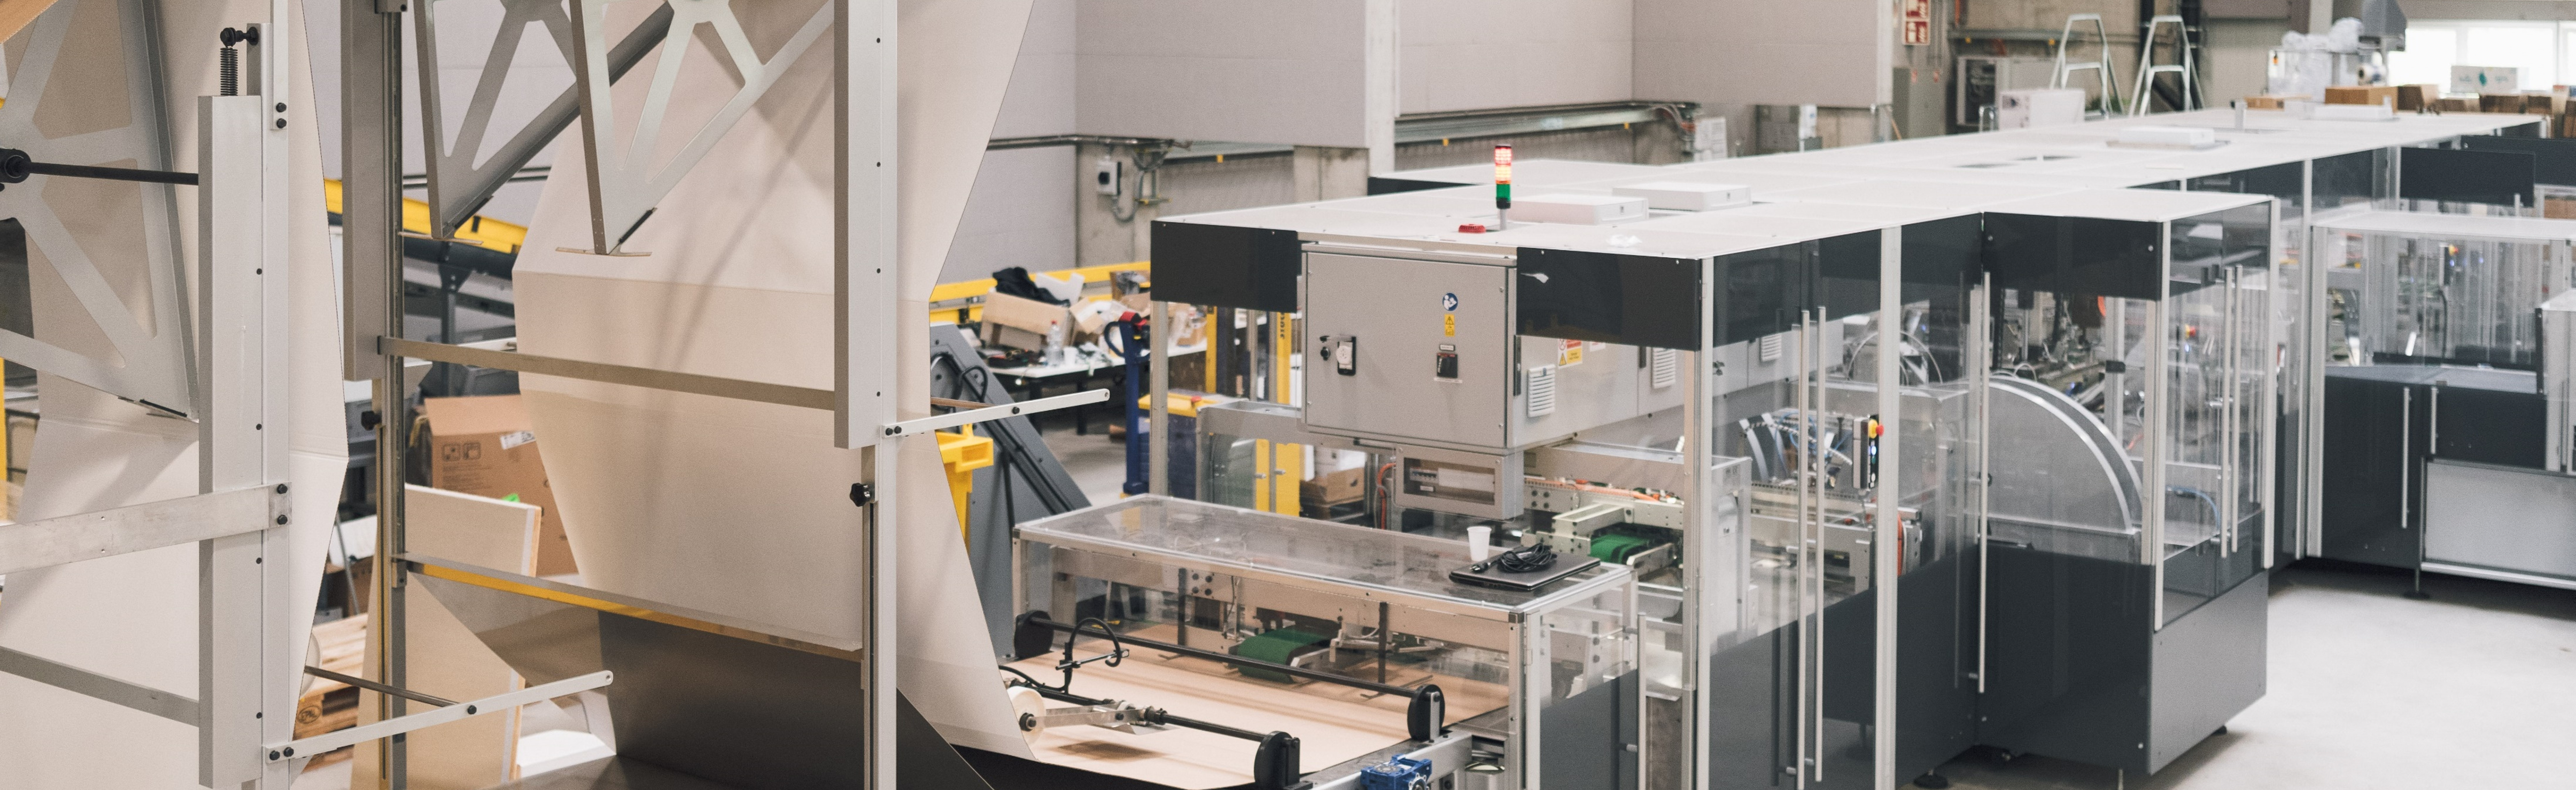
\includegraphics[width=17.5cm]{logovpm}
}
% can also use any field given by \author, \title, \date, \institute, or \tikz to place image in the title page
%\addtobeamertemplate{headline}{}{% on each slide with headline
%    \tikzart[t=p,x=8,y=7,w=4]{logo_uw}
%}
%---------------------------------------------------------------------------%
%
\begin{document}
\begin{frame}[plain]
    \titlepage%
    %\tikzart[t=p,x=0,y=-4,w=4]{logo_uw}
    \addtocounter{framenumber}{-1}% modify the counter to exclude a frame from total count
\end{frame}%
\section{Produzierte Boxen}
\begin{frame}
    \frametitle{Produzierte Pakete pro Tag}
    \begin{figure}
        \centering
        \includegraphics[width=0.80\pagewidth]{single_linechart_pb_tot}
    \end{figure}
\end{frame}

\begin{frame}
    \frametitle{Produzierte Pakete pro Tag und Maschine}

    \begin{figure}
        \centering
        \includegraphics[width=0.80\pagewidth]{daily_barplot_pb}
    \end{figure}

\end{frame}

\begin{frame}
    \frametitle{Total produzierte Boxen}

    \begin{figure}
        \centering
        \includegraphics[width=0.80\pagewidth]{donut_chart_total_box_pm}
    \end{figure}

\end{frame}

% TODO: lower graphic scaling to match frame size
\begin{frame}
    \frametitle{Total produzierte Pakete pro Monat}

    \begin{figure}
        \centering
        \includegraphics[width=0.80\pagewidth ]{historic_single_bar_total}
    \end{figure}

\end{frame}%
\section{Pakete pro Stunde}

\begin{frame}
    \frametitle{Produzierte Pakete pro Stunde}

    \begin{figure}
        \centering
        \includegraphics[width=0.75\pagewidth]{multiline_daily_tp}
    \end{figure}

\end{frame}

\begin{frame}
    \frametitle{Durchschnitt pro Stunde und Maschine}

    \begin{figure}
        \centering
        \includegraphics[width=0.75\pagewidth]{multibar_monthly_tp}
    \end{figure}

\end{frame}

\begin{frame}
    \frametitle{Produzierte Pakete pro Stunde - CMC}

    \begin{figure}
        \centering
        \includegraphics[width=0.75\pagewidth]{multiline_daily_tp_cmc}
    \end{figure}

\end{frame}

\begin{frame}
    \frametitle{Durchschnitt pro Stunde und Maschine - CMC}

    \begin{figure}
        \centering
        \includegraphics[width=0.75\pagewidth]{multibar_monthly_tp_cmc}
    \end{figure}

\end{frame}
\section{Status der Maschinen}
\begin{frame}
    \frametitle{Status der Maschinen - Total}

    \begin{figure}
        \centering
        \includegraphics[width=0.80\pagewidth]{pie_chart_total}
    \end{figure}

\end{frame}

%TODO: change image scaling to better fit the columns/frame
\begin{frame}
    \frametitle{Status pro Maschine}

    \begin{columns}[t]
        \begin{column}{0.48\linewidth}
            \begin{figure}
                \centering
                \includegraphics[width=0.45\pagewidth]{pie_chart_L1 - VPM B (4958)}
            \end{figure}
        \end{column}
        \begin{column}{0.48\linewidth}
            \begin{figure}
                \centering
                \includegraphics[width=0.45\pagewidth]{pie_chart_L2 - VPM A (4959)}
            \end{figure}
        \end{column}
    \end{columns}

\end{frame}

\begin{frame}
    \frametitle{Status pro Maschine}

    \begin{columns}[t]
        \begin{column}{0.48\linewidth}
            \begin{figure}
                \centering
                \includegraphics[width=0.45\pagewidth]{pie_chart_L3 - VPM C (4960)}
            \end{figure}
        \end{column}
        \begin{column}{0.48\linewidth}
            \begin{figure}
                \centering
                \includegraphics[width=0.45\pagewidth]{pie_chart_L4 - VPM D (4961)}
            \end{figure}
        \end{column}
    \end{columns}

\end{frame}
\section{Bad Boxes}
\begin{frame}
    \frametitle{Bad Boxes pro Tag}

    \begin{figure}
        \centering
        \includegraphics[width=0.75\pagewidth]{lineplot_daily_abs_bad_boxes}
    \end{figure}

\end{frame}

\begin{frame}
    \frametitle{Bad Boxes absolut pro Maschine und Tag}

    \begin{figure}
        \centering
        \includegraphics[width=0.75\pagewidth]{groupedbar_daily_abs_bad_boxes}
    \end{figure}

\end{frame}

\begin{frame}
    \frametitle{Bad Boxes relativ pro Maschine und Tag}

    \begin{figure}
        \centering
        \includegraphics[width=0.75\pagewidth]{groupedbar_daily_rel_bad_boxes}
    \end{figure}

\end{frame}

\begin{frame}
    \frametitle{Bad Boxes relativ pro Maschine}

    \begin{figure}
        \centering
        \includegraphics[width=0.75\pagewidth]{multibar_monthly_rel_bad_boxes}
    \end{figure}

\end{frame}
\section{Verfuegbarkeit}
\begin{frame}
    \frametitle{Verfuegbarkeit}

    \begin{figure}
        \centering
        \includegraphics[width=0.80\pagewidth]{daily_barplot_op_avail}
    \end{figure}

\end{frame}

\begin{frame}
    \frametitle{Durchschnittliche Verfuegbarkeit}

    \begin{figure}
        \centering
        \includegraphics[width=0.80\pagewidth]{historic_multi_avg_avail}
    \end{figure}

\end{frame}
\end{document}
%---------------------------------------------------------------------------%
